\chapter{Importance Sampling Approach to Chance Constrained DC-OPF}
This chapter is based on the publication of the dissertation author: Importance Sampling Approach to Chance-Constrained DC Optimal Power Flow / Lukashevich, A., Gorchakov, V., Vorobev, P., Deka, D., \& Maximov, Y. //IEEE Transactions on Control of Network Systems. 2023. Vol. 11, no. 2. P. 928-937.
\label{chap:dc_stochastic_approx}

\section{Introduction}

In 2020 electricity produced approximately 25\% of greenhouse gas emissions in the USA, and integration of a higher volume of renewable energy generation is seen as the primary tool to reduce the emission level \cite{hockstad2018inventory}. In turn, a higher amount of renewable generation increases the power grid uncertainty, compromises its security, and challenges classical power grid operation and planning policies \cite{koutsoyiannis2016unavoidable}. 

The optimal power flow (OPF) problem, which determines the economically optimal operating level of power generation under given power balance equations and security constraints, is one of the most fundamental problems in grid operation and planning \cite{stott2012optimal}. Several extensions are proposed for the optimal power flow problem for addressing the uncertainty of power generation and consumption \cite{geng2019data}. Robust and chance-constrained power flow formulations are among the most popular ones. The robust OPF problem assumes bounded uncertainty and requires a solution to be feasible against any possible uncertainty realization within a given uncertainty set~\cite{ben2002robust,ding2016adjustable,sousa2010robust}. 

A more flexible and general chance-constrained approach requires security constraints to be satisfied a high probability while assuming the distribution of renewables is known in whole or in part \cite{lubin2015robust, roald2017chance,bienstock2014chance,pena2020dc,mitrovic2023gp,mitrovic2023data}. We consider a joint chance-constrained optimal power flow problem, where the joint probability of at least one failure of the security constraints (line load limits, voltage stability bounds) is bounded from above by a confidence threshold (JCC-OPF). 

In contrast to a single chance-constrained formulation (SCC-OPF), which imposes individual failure probability thresholds for each of the constraints, the joint chance constraint is computationally hard even for direct current (DC) power balance equations, which is characterized by linear security limits, with Gaussian uncertainty~\cite{cousins2014cubic,khachiyan1993complexity}. Several tractable convex approximations have been proposed \cite{nemirovski2007convex, nemirovski2006scenario,nemirovski2003tractable,trofino1999bi} for joint chance-constrained optimization to overcome the computational hardness of the problem. However, they often lead to conservative solutions inapplicable for operational practice. 

Other approaches such as scenario and sample average approximations \cite{calafiore2006scenario,garatti2019risk, vrakopoulou2013probabilistic,nemirovski2006scenario} consist of substituting the stochastic part with a set of deterministic inequalities based on the uncertainty realization. This approach can be distributionally robust and allow exploiting uncertainties beyond the Gaussian ones. A combination of an analytical approximation and sampling~\cite{hou2020chance} can further improve the accuracy of the solution. However, it may require a large number of samples. Scenario curation/modification heuristics have been designed to improve the sample complexity of JCC-OPF \cite{mezghani2020stochastic}, although without formal analysis of the methodology. In work outside power grids, statistical learning has been used to approximate uncertain convex programs~\cite{vapnik1999overview,maximov2016tight,campi2020scenario}.

Nevertheless, the scenario approximation approach remains the most accurate algorithm for solving the joint chance-constrained DC optimal power flow. At the same time, its complexity is often unacceptable for large-scale power grids~\cite{sakhavand2020new}. To this end, the study suggests using importance sampling to reduce the complexity and improve the accuracy of the scenario approximation to chance-constrained optimal power flow. The importance sampling approach generates more informative samples and results in an optimization problem with fewer constraints. Our study extends earlier results \cite{barrera2016chance,tong2022optimization} on importance sampling for chance-constrained optimization. 

The contribution of the study is as follows. 
\begin{enumerate}
  \item we propose a novel computationally efficient 
  approach to the joint chance-constrained DC OPF problem. The algorithm exploits physics-informed importance sampling to refine the classical scenario approximation~\cite{calafiore2006scenario};
  \item we prove the algorithm to converge to a solution of JCC-DC-OPF with a guaranteed accuracy under mild technical assumptions; 
  \item we demonstrate the proposed algorithm's superior computational efficiency and accuracy relative to standard methods over multiple real and synthetic test cases.
\end{enumerate}

The chapter is organized as follows.
Section~\ref{sec:not-dc} presents the joint chance-constrained optimal power flow problem and introduces the notation used in the chapter. We outline the algorithm and provide its theoretical analysis in Section~\ref{sec:algo-dc}. Empirical study and comparison to state-of-the-art methods are given in Section~\ref{sec:emp-dc}. In Section~\ref{sec:conclusion-dc} we conclude with a summary and critical discussion on possible applications of our results.



\section{Background and Problem Setup}\label{sec:not-dc}

\subsection{Notation}
The direct current (DC) power flow approximation remains extremely popular yet simple model for analysis because of a linear relation between powers and phase angles in typical high-voltage power grids. 

In this study, we consider a power grid given by a graph $\mathcal{G} = (V, E)$ with a set of nodes/buses $V$ and edges/lines $E$. Assume $n+1$ is a number of buses, and $m$ is a number of lines. Let $p$ be a vector of power injections $p = (p_F, p_R, p_S)^\top$, where $p_F$ corresponds to buses with deterministic/fixed (F) power injections, $p_R$ to buses with random (R) injections, and $p_S$ is the injection at the slack bus (S). The power system is balanced, i.e., the sum of all power injections equals to zero, $p_S = -\sum_{r\in R} p_r - \sum_{f\in F} p_f$. Let $B \in \mathbb{R}^{n+1 \times n+1}$ be an admittance matrix of the system, $p = B\theta$. The components $B_{ij}$ are such that $B_{ij} \neq 0$ if there is a line between nodes $i$ and $j$, the diagonal elements $B_{ii} = - \sum_{j\neq i} B_{ij}$, i.e., $B$ is a Laplacian matrix. Let $\theta$ be a vector of phase angles. Thus, $B$ is rank deficient with one eigenvalue equal to $0$. Without a loss of generalization, we assume that the phase angle on the reference slack bus $\theta_S = 0$, and given that the injection $p_S$ is the negative sum of the other injections, we can analyze a \textit{reduced} order system by ignoring the reference bus $S$. This is done by removing the injection and phase angle at $S$ from $p$ and $\theta$, and removing the row and column corresponding to $S$ from $B$. This gives an invertible reduced power-flow model at the non-reference buses \cite{aburbook,dekatcns}. We use $\theta, p, B$ to the reduced quantities and can write their inverse relation as ~$\theta = B^{-1} p$.

The DC power flow equations, generation and stability constraints are
\begin{align}
    & p = B \theta \label{eq:DC-PF-a-dc}\\
    & p^{\min}_i \leq p_i \leq p^{\max}_i, i \in V \label{eq:DC-PF-b-dc}\\
    & |\theta_i - \theta_j| \leq \bar{\theta}_{ij}, \; (i,j)\in E \label{eq:DC-PF-c-dc}
\end{align}
Let $A \in \{-1,0,1 \}^{m \times n}$ be the reduced incidence matrix, i.e., column corresponding to reference bus $S$ is removed, of grid $G$. If nodes $i$ and $j$ are connected by edge $k$ then $A_{ki} = +1$, $A_{jk} = -1$ and all other elements are equal to zero. Then the phase angle constraints in \eqref{eq:DC-PF-c-dc} can be represented as  $AB^{-1}p \le \bar\theta$, $-AB^{-1}p \le \bar\theta$. 

%Let $C \in \mathbb{R}^{n\times n}$ be a symmetric matrix such that for all random nodes $r$, fixed nodes $f$ and the slack node $S$, $C_{rr} = 1$, $C_{ff} = 1$, $C_{Sr} = - 1$, $C_{Sf} = - 1$, while all other elements are equal to zero. 
In DC OPF (Optimal power Flow), we seek to minimize some cost (linear or quadratic), denoted as $\textit{cost}(p)$ on power injections such that the following system of inequalities (operational constraints) are satisfied: 
%{\color{red} \emph{In the description right after formulation (5), the authors assume that the generation cost $\textup{cost}(x,\xi)$ does not depend on the randomness but may depend on the uncertainty distribution. It is a bit confusing to me. Can the authors further explain or give an example to elaborate with more details?}: might be reasonable to address that question here}
\[
\underbrace{(AB^\dagger, - A B^\dagger, I, -I)}_{W}\!\!{}^\top p \le \underbrace{(\bar\theta, \bar\theta, p_{\max}, -p_{\min})}_b\!\!{}^\top,
\]
where $I$ is $n\times n$ identity matrix. Let $J$ be a number of constraints, $J = 2m + 2n$, then $W\in\mathbb{R}^{J\times n}$ and $b\in\mathbb{R}^{n\times 1}$. We refer to the feasibility polytope as the set~$\mathcal{P}$, 
$\mathcal{P} = \bigl\{p:\, Wp \le b\bigr\} = \bigl\{p:\; \bigcap_{i=1}^J\omega_i^\top p \le b_i\bigr\}$.

Finally, we assume that fluctuations of power injections $p$ are Gaussian, $p = x +\xi$, where $\xi$ is a zero mean Gaussian uncertainty, $\xi\sim\mathcal{N}(0, \Sigma)$ and $x$ is the deterministic part of power injections. Under this setting, we solve a joint chance-constrained OPF problem, where the DC-OPF cost is replaced by the expected value $\mathbb{E}_{\sim \xi}\textit{cost}(x,\xi)$ and the operational constraints are now satisfied probabilistically, instead of exactly. This is described in the next section.
% \begin{align}\label{eq:JCC-OPF}
%   \min_x & \;\mathbb{E}_{\xi\sim \mathcal{N}(0, \Sigma)}

The chapter notation is summarized in Table~\ref{tab:notation-dc}. We use lower indices for coordinates of vectors and matrices, lower-case letters for probability density functions (PDFs), and upper-case letters for cumulative distribution functions (CDFs). When it does not lead to a confusion, we use $\mathbb{P}$ and $\mathbb{E}$ to denote probability and expectation without explicitly mentioning a distribution. 

\begin{table}[t]
  \caption{Chapter notation. }
  \centering
  \begin{tabularx}{\textwidth}{|m{1cm}|X|m{1.5cm}|X|}
  % \begin{tabular}{|p{1.15cm}|p{4.95cm}|p{1.35cm}|p{4.85cm}|}
    \toprule \\
    $\mathcal{D}$  & $\xi \sim \mathcal{N}(0, \Sigma), ~\xi \notin \mathcal{P}_{\texttt{in}}$ & $\nu(p)$ & $\textup{PDF}_{\mathcal{N}(0, \Sigma)}$ w/o $\mathcal{P}_{\texttt{in}}$ in support \\
    $E$    & set of lines & $q_{D_i}(\xi)$ & mix. component PDF \\
    $V$ & set of buses & $q_D(\xi)$ & mix. distribution PDF \\
    $B$ & admittance matrix& $p^{\max}$ & generation upper limits \\
    $m$ & number of lines & $p^{\min}$ & generation lower limits \\
    $n$ & number of buses & $\mathbb{P}$, $\mathbb{E}$ & probability, expectation \\
    $p$ & power injections & $\mathcal{P_{\texttt{in}}}$ & redundant scen. polytope \\
    $\theta$ & voltage phases & $\mathcal{N}(\cdot, \cdot)$ & Gaussian distribution \\
    $I_n$ & $n\times n$ identity matrix & $\mathcal{P} $ & feas. set  $\{p: Wp\leq b \}$ \\
    $J$ & number of constraints &  $x$ & det. injection $x = \mathbb{E}_\xi p$ \\
    $\bar\theta_{ij}$ & voltage angle limits & $\pi$ & $\mathbb{P}\{\xi \in \mathcal{P}_{\texttt{in}}\}$ \\
    $\xi$ & $\sim\mathcal{N}(0, \Sigma)$ stoch. inj. & $\delta$  & reliability of SA solution \\ 
    $\mathcal{P}_{out}$   & JCC outer approx.  & $\eta$  & confidence level \\
    \bottomrule
  \end{tabularx}
  \label{tab:notation-dc}
\end{table}

\subsection{Problem Setup}
The joint chance-constrained optimal power flow problem~is:
\begin{equation}\label{eq:JCC-OPF-dc}
    \begin{aligned}
  \min_x & \;\mathbb{E}_{\xi\sim \mathcal{N}(0, \Sigma)} \textit{cost}(x,\xi)\\
   \textit{s. t. }\; & \mathbb{P}_{\xi\sim \mathcal{N}(0, \Sigma)} (x+\xi \in \mathcal{P}) \ge 1 - \eta
   \end{aligned}
\end{equation}
where $\eta$ is a preset confidence parameter with $0 < \eta \le 1/2$, and $\textit{cost}(x, \xi)$ is a cost function convex in $x$ for any realization of $\xi$. In other words, we assume that power flow balance equations (Eqs.~\eqref{eq:DC-PF-a-dc}) are satisfied almost surely, and the probability that at least one of the security constraints (Eqs.~\eqref{eq:DC-PF-b-dc} and~\eqref{eq:DC-PF-c-dc}) fails is at most $\eta$. 

Notice that despite the convexity of the cost function of Problem~\eqref{eq:JCC-OPF-dc} is non-convex as its feasibility set is non-convex for a low level of target confidence, i.e., $\eta < 0.5$.

\subsection{Scenario Approach}

Over the last two decades, the scenario approach \cite{nemirovski2006scenario,calafiore2006scenario} 
remains the state-of-the-art method for solving joint chance-constrained optimization. The scenario approach consists in substituting the probabilistic constraints with a large number of deterministic ones with each constraint standing for some uncertainty realization:
\begin{align}\label{eq:sc-opf-dc}
  \min_x & \; \frac{1}{N} \sum_{t=1}^N \textit{cost}(x,\xi^t)\\
  \textit{s. t. } & \; p^{\min} \le x+\xi^t \le p^{\max}, \; 1\le t \le N\nonumber\\
  & \; |\theta_i(\xi^t) - \theta_j(\xi^t)| \le {\bar \theta}_{ij}, (i, j)\in \mathcal{E}, \; 1\le t \le N\nonumber\\
  & x+\xi^t = B \theta(\xi^t), \; 1\le t \le N\nonumber
\end{align}
where $N$ is a number of scenarios, and $\{\xi^t\}_{i=1}^N$ is a set of uncertainty realization. We assume below that the generation cost function $\textit{cost}(x, \xi)$ does not depend on the randomness in power fluctuation ($\textit{cost}(x, \xi) = \textit{cost}(x)$ for any uncertainty realization $\xi$), but may depend on the uncertainty distribution (i.e., on its mean or variance). %{\color{red} Note that dependence of expected cost on known asymptotic parameters of the distribution (variance, mean) are allowed within this framework.}

The key disadvantage of the scenario approximation \eqref{eq:sc-opf-dc} is the number of constraints induced by adding scenarios $\xi^t$. A classical theory, developed by Calafiore and Campi \cite{calafiore2006scenario}, suggests to include a large number of scenarios $N$. This will allow the solution of \eqref{eq:sc-opf-dc} to be feasible for original problem \eqref{eq:JCC-OPF-dc} with high probability $1 - \delta$. However, the number of required scenarios $N$ is given by $N \geq 2 \left( \frac{\ln{1/\delta}}{\eta} + d + d\frac{\ln{1/\eta}}{\eta} \right)$, where $d$ is the number of control variable in the optimization problem. For example, with $\eta = 10^{-2}, \delta = 10^{-2}$, for  IEEE-57 case one would end up with $6.45 \cdot 10^3$ (6 generators, excluding slack one) constraints which is time- and memory-consuming to solve.
% \yury{Is that correct?}
% \sasha{Why not? I have estimated these numbers using Campi's theorem and used number of constraints from IEEE-54}

The major contribution of this chapter is a significant reduction of the requirement on the number of samples by sampling the most informative scenarios. The latter reduces the computational complexity of the scenario approximation and comes up with tight accuracy guarantees for the joint chance-constrained DC optimal power flow problem. 

% and keeping the theoretical guarantees. It is achieved by picking samples from distribution that does not contain ''weak'' samples within its domain. Next, we show that solving scenario approximation with those samples provides better theoretical guarantees on the number of samples - $N$ and the probability to obtain feasible solution of original JCC problem is  $1 - \beta$.
% We next discuss our method to solve Problem \eqref{eq:sc-opf}.

\section{Algorithm}\label{sec:algo-dc}

\subsection{Idea and Sketch}
Our algorithm consists of several steps: 
(1) constructing an inner approximation to the feasibility set,
(2) generating samples outside of this approximation,
(3) and, finally, solving the scenario approximation Problem \eqref{eq:sc-opf-dc} with the generated collection of samples.

First, using the fact that \emph{the probability of a union of events is bounded from below by the maximum of individual event probabilities}, we construct a lower bound on the probability of constraint feasibility $\mathbb{P}(x+\xi \in \mathcal{P})$. The latter allows to add a set of constraints, $x\in \mathcal{P}_{out}$, so that if $x\not\in \mathcal{P}_{out}$ then $\mathbb{P}(x+\xi \notin \mathcal{P}) > \eta$. In other words, if the solution $\bar x$ of the scenario approximation~ \eqref{eq:sc-opf-dc} with samples from the nominal distribution $\mathcal{N}(0,\Sigma)$ satisfies $\mathbb{P}(x+\xi \in \mathcal{P}) \ge 1-\eta$, then adding additional inequalities $x\in \mathcal{P}_{out}$ does not change $\bar x$. Second, using the aforementioned bound, we design a polytope $\mathcal{P}_{\texttt{in}}(x) = \{p: W_{\texttt{in}} \xi \le b_{\texttt{in}}, p = x+\xi\}$ around $x$ with $W_{\texttt{in}}$ and $b_{\texttt{in}}$ independent of $x$. We present the exact expressions for $W_{\texttt{in}}$ and $b_{\texttt{in}}$ in Theorem \ref{thm:20-dc}. Figure~\ref{fig:10-dc} illustrates the idea. We consider a deterministic feasibility set $\mathcal{P}$ and derive a polytope $\mathcal{P}_{out}$ inside of it so that no optimal solution $x^*$ of Prob.~ \eqref{eq:JCC-OPF-dc} belongs to $\mathcal{P}\setminus \mathcal{P}_{out}$. The polytope $\mathcal{P}_{\texttt{in}}(x)$ depicts the distances between the planes of $\mathcal{P}$ and $\mathcal{P}_{out}$ for each $x$.
%The polytope $\mathcal{P}_{\texttt{in}}$, defined in terms of noise $\xi$ only, $.
Samples of uncertainty outside $\mathcal{P}_{\texttt{in}}(0)$ are used to determine an optimal solution using importance sampling, which will be discussed in detail in Section~\ref{sec:obs-dc}.

Then, we show that for any sample $\xi^t$ and feasible $x$, if $p = x+\xi^t \in \mathcal{P}_{\texttt{in}}(x)$, then $p$ also necessarily belongs to the constraint feasibility set $\mathcal{P}$. To this end scenarios $\xi^t: x+\xi^t \in \mathcal{P}_{\texttt{in}}$ can be eliminated from the optimization problem (see Eq.~\eqref{eq:sc-opf-dc}) without impacting the approximation accuracy. 
\def\shift{2.7}
\def\shiftt{2.35}
\def\shiftuselesssample{0.3}
\def\shiftusefulsample{1.1}
\begin{figure}
    \centering
        \begin{tikzpicture}[scale=0.75, node distance={15mm}, thick, main/.style = {draw, scale=.9}] 
        %x
        \coordinate (x) at (0, 0);
        \draw (x) circle (1pt);
        \draw (x) ++(0.05, 0.05) node[above right] (tmp) {$x$};
        %x2
        \coordinate (x2) at (0 + \shiftt, 0 - \shiftt);
        \draw (x2) circle (1pt);
        \draw (x2) ++(0.05, 0.05) node[above right] (tmp) {$x^*$};
        %outer guy
        \coordinate (a) at ( 4.755282581475767 , 1.545084971874737 );
        \coordinate (b) at ( 3.061616997868383e-16 , 5.0 );
        \coordinate (c) at ( -4.755282581475767 , 1.5450849718747375 );
        \coordinate (d) at ( -2.9389262614623664 , -4.045084971874736 );
        \coordinate (e) at ( 2.9389262614623646 , -4.045084971874738 );
        %linking outer guy
        \draw (a) -- (b);
        \draw (b) -- (c);
        \draw (c) -- (d);
        \draw (d) -- (e);
        \draw (e) -- (a);
        %annotating outer guy
        \draw
        (a) ++(0.1, 0.01) node[above] (tmp) {$\mathcal{P}$};
        %(tmp.west) -- (PO);
        
        %green guy
        \coordinate (ag) at ( 3.804226065180614 , 1.2360679774997896 );
        \coordinate (bg) at ( 2.4492935982947064e-16 , 4.0 );
        \coordinate (cg) at ( -3.804226065180614 , 1.23606797749979 );
        \coordinate (dg) at ( -2.351141009169893 , -3.2360679774997894 );
        \coordinate (eg) at ( 2.3511410091698917 , -3.2360679774997902 );
        %linking green guy
        \draw [olive] (ag) -- (bg);
        \draw [olive] (bg) -- (cg);
        \draw [olive] (cg) -- (dg);
        \draw [olive] (dg) -- (eg);
        \draw [olive] (eg) -- (ag);
        %annotating green guy
        \draw
        (bg) ++(0.1, 0.01) node[below, olive] (tmp) {$\mathcal{P}_{out}$};
        %(tmp.west) -- (PO);
        
        %red guy
        \coordinate (ar) at ( 0.9510565162951535 , 0.3090169943749474 );
        \coordinate (br) at ( 6.123233995736766e-17 , 1.0 );
        \coordinate (cr) at ( -0.9510565162951535 , 0.3090169943749475 );
        \coordinate (dr) at ( -0.5877852522924732 , -0.8090169943749473 );
        \coordinate (er) at ( 0.5877852522924729 , -0.8090169943749476 );
        %linking red guy
        \draw [red] (ar) -- (br);
        \draw [red] (br) -- (cr);
        \draw [red] (cr) -- (dr);
        \draw [red] (dr) -- (er);
        \draw [red] (er) -- (ar);
        %annotating red guy
        \draw
        (br) ++(1em, .1em) node[above right, red] (tmp) {$\mathcal{P}_{\texttt{in}}(x)$};
        %(tmp.west) -- (PO);
        
        %red guy2
        \coordinate (ar2) at ( 0.9510565162951535 + \shiftt , 0.3090169943749474 - \shiftt);
        \coordinate (br2) at ( 6.123233995736766e-17 + \shiftt , 1.0  - \shiftt);
        \coordinate (cr2) at ( -0.9510565162951535  + \shiftt, 0.3090169943749475  - \shiftt);
        \coordinate (dr2) at ( -0.5877852522924732 + \shiftt, -0.8090169943749473 - \shiftt);
        \coordinate (er2) at ( 0.5877852522924729 + \shiftt, -0.8090169943749476  - \shiftt);
        %linking red guy
        \draw [red] (ar2) -- (br2);
        \draw [red] (br2) -- (cr2);
        \draw [red] (cr2) -- (dr2);
        \draw [red] (dr2) -- (er2);
        \draw [red] (er2) -- (ar2);
        %annotating red guy
        \draw
        (br2) ++(1em, .1em) node[above, red] (tmp) {$\mathcal{P}_{\texttt{in}}(x^*)$};
        %(tmp.west) -- (PO);
        
        %Upper \Delta_i
        \coordinate (b_) at (1, 5.7265);
        \draw
        (b_) node[above right] (tmp) {$\Delta_i$};
        %(tmp.west) -- (PO);
        \coordinate (bg_) at (1.5, 5.0898);
        \draw [dashed] (b) -- (b_);
        \draw [dashed] (bg) -- (bg_);
        \draw [thick, black, -latex'] (b_) -- (bg_);
        \draw [thick, black, -latex'] (bg_) -- (b_);
        
        %Inner \Delta_i
        \coordinate (br_) at (-1.5, -0.0898137920080413);
        \draw
        (br_) node[above left] (tmp) {$\Delta_i$};
        %(tmp.west) -- (PO);
        \coordinate (x0_) at (-1.0, -0.7265425280053608);%x!
        \draw [dashed] (br) -- (br_);
        \draw [dashed] (x) -- (x0_);
        \draw [thick, black, -latex'] (br_) -- (x0_);
        \draw [thick, black, -latex'] (x0_) -- (br_);
        
        %Inner \Delta_i 2
        \coordinate (br_2) at (-1.5 + \shiftt, -0.0898137920080413 - \shiftt);
        \draw
        (br_2) node[above left] (tmp) {$\Delta_i$};
        %(tmp.west) -- (PO);
        \coordinate (x0_2) at (-1.0 + \shiftt, -0.7265425280053608-  \shiftt);%x!
        \draw [dashed] (br2) -- (br_2);
        \draw [dashed] (x2) -- (x0_2);
        \draw [thick, black, -latex'] (br_2) -- (x0_2);
        \draw [thick, black, -latex'] (x0_2) -- (br_2);
        
        % Samples
        %% Useless
        \coordinate (xu_1) at (\shiftt + \shiftusefulsample * 0.1, -\shiftt - 3.5*\shiftuselesssample);
        \draw [teal] (xu_1) circle (1pt);
        \coordinate (xu_2) at (\shiftt + \shiftusefulsample, -\shiftt + \shiftusefulsample * 0.5);
        \draw [teal] (xu_2) circle (1pt);
        \coordinate (xu_3) at (\shiftt - \shiftusefulsample * 0.2, -\shiftt + \shiftusefulsample);
        \draw [teal] (xu_3) circle (1pt);
        \coordinate (xu_4) at (\shiftt + \shiftusefulsample * 0.7, -\shiftt - \shiftusefulsample);
        \draw [teal] (xu_4) circle (1pt);
        \end{tikzpicture}  
   
%   \caption{We consider an operating point $x$ and derive a polytope $\mathcal{P}_{out}$ (over the mean level of power injections, $x$) so that no optimal solution $x^*$ of Prob.~ \eqref{eq:JCC-OPF} belongs to $x^*\in\mathcal{P}\setminus \mathcal{P}_{out}$. As it is shown on the figure, polytope $\mathcal{P}_{out}$ (over $x$) induces a polytope $\mathcal{P}_{\texttt{in}}$ (over power injections $p$, $p = x + \xi$) so that none of uncertainty realizations $\xi$ s.t. $p = x+\xi\in\mathcal{P}_{\texttt{in}}$ affect the scenario approximation solution. }

\caption{Interrelation between deterministic feasibility set, JCC feasibility set and as sampling polytopes.}
  \label{fig:10-dc}
  %\vspace
\end{figure}

Finally, we sample scenarios outside of the polytope $\mathcal{P}_{\texttt{in}}$ using the state-of-the-art importance sampling methods \cite{owen2019importance,lukashevich2021power} and solve the Scenario Approximation Problem~\eqref{eq:sc-opf-dc} with the collection of samples generated from importance distribution. Later in this section, we provide rigorous proof of the algorithm's efficiency and justify its empirical performance in Section~\ref{sec:emp-dc}. 

\subsection{Inner Approximation}

Consider a probability for the power generation $p$ of being inside the feasibility polytope, $p\in \mathcal{P}$:
\begin{align*}
  \mathbb{P}&(p\in \mathcal{P}) = 
  \mathbb{P}(p: Wp \le b) = \\
  & \mathbb{P}\left(p: \bigcap_{i=1}^J \omega_i^\top p \le b_i\right) = 1 - \mathbb{P}\left(p: \bigcup_{i=1}^J \omega_i^\top p > b_i\right)\le\\
  %
  & 1 - \max_{1\le i\le J}\mathbb{P}\left(p: \omega_i^\top p > b_i\right).
\end{align*}

So, if there exists $x$ such that for some $i$, $\mathbb{P}(\omega_i^\top p > b_i) > \eta$, then $\mathbb{P}(p\in \mathcal{P}) < 1-\eta$. Thus, to satisfy the joint chance constraint for $p = x+\xi$, $\xi\sim \mathcal{N}(0, \Sigma)$, we need

\begin{align}
  \eta \;\ge\; & \mathbb{P}(\omega_i^\top p > b_i) = \mathbb{P}(\omega_i^\top \xi + \omega_i^\top x > b_i) = \nonumber\\
  & 
  \mathbb{P}\left(\frac{\omega_i^\top \xi}{\|\Sigma^{1/2}\omega_i\|_2} > \frac{b_i - \omega_i^\top x}{\|\Sigma^{1/2}\omega_i\|_2}\right) = \nonumber\\
  & \mathbb{P}\left(\zeta > \frac{b_i - \omega_i^\top x}{\|\Sigma^{1/2}\omega_i\|_2}\right) = \Phi\left(\frac{\omega_i^\top x - b_i}{\|\Sigma^{1/2}\omega_i\|_2}\right), \label{eq:cnv-dc}
\end{align}

where $\zeta\sim \mathcal{N}(0,1)$, $\Phi$ is the CDF of the standard normal distribution. Notice, that the function $\Phi(\cdot)$ is convex if its argument is negative, consequently, Ineq.~\eqref{eq:cnv-dc} is convex if~$x\in \mathcal{P}$. 

A set of inequalities $\eta \ge \Phi\left((\omega_i^\top x - b_i)/(\|\Sigma^{1/2}\omega_i\|_2)\right)$, $1\le i \le J$, defines a polytope $\mathcal{P}_{out}$ as follows: 

\begin{align}\label{eq:05-dc}
  P_{out} = \left\{x: \omega_i^\top x \le b_i - \Delta_i, 1\leq i\leq J\right\},
\end{align}

where $\Delta_i = \|\Sigma^{1/2}\omega_i\|_2 \Phi^{-1}(1-\eta)$, $\eta \le 1/2$. %In other words, the operational point $x$ can not be too close to the feasibility boundary to meet the security constraints with a high probability. 
Figure~\ref{fig:10-dc} illustrates mutual arrangement of the polytopes $\mathcal{P}_{out} \subset\mathcal{P}$. Note that $\mathcal{P}_{out}$ defines an outer approximation of the chance-constrained feasibility set, which is itself an inner approximation of the constraint feasiblity set without any uncertainty. Eq.~\eqref{eq:05-dc} implies 
Theorem~\ref{thm:10-dc}.
\begin{theorem}\label{thm:10-dc}
  The joint chance-constrained optimal power flow problem~ \eqref{eq:JCC-OPF-dc} has the same set of optimal solutions as 
  \begin{align}\label{eq:JCC-OPF-Ad-dc}
  \min_x & \;\mathbb{E}_{\xi\sim \mathcal{N}(0, \Sigma)} \textit{cost}(x,\xi)\\
   \textit{s. t. }\; & \mathbb{P}_{\xi\sim \mathcal{N}(0, \Sigma)} (x+\xi \in \mathcal{P}) \ge 1 - \eta, 0 < \eta \le 1/2,\nonumber\\
   & \; x\in \mathcal{P}_{out}\nonumber 
\end{align}
\end{theorem}
\begin{proof}
%{\color{red}Sasha \& Slava, pls add a proof, almost just a refs to Eq.~\eqref{eq:05}.}
A set of additional equations $x\in\mathcal{P}_{out}$ does not affect the solution of Problem~$\eqref{eq:JCC-OPF-dc}$ because the feasiblity set of the chance-constrained optimization problem is inside $\mathcal{P}_{out}$, since the probability for a scenario to be outside of the polytope $\mathcal{P}$ is lower bounded by the probability of being outside of its single face. The latter determines polytope $\mathcal{P}_{out}$, see. Eq.~\ref{eq:05-dc} for details. 
%Eq.~\eqref{eq:05} implies that any optimal solution of  \eqref{eq:JCC-OPF} is also a solution to  \eqref{eq:JCC-OPF-Ad} according to the definition of $\mathcal{P}_{out}$. Moreover, any solution of the Problem~ \eqref{eq:JCC-OPF-Ad} is feasible for Problem~ \eqref{eq:JCC-OPF} and have the same objective. The latter implies that the sets of solutions for~ \eqref{eq:JCC-OPF} and~ \eqref{eq:JCC-OPF-Ad} are the same. 
%
%First, a set of the optimal solutions of \ref{eq:JCC-OPF-Ad} with additional deterministic constraints $x\in \mathcal{P}_{out}$ is a subset of the set of solution of \ref{eq:JCC-OPF}. In this case, according to the definition of $\mathcal{P}_o$, the optimal solution is inside of $\mathcal{P}_o$. Thus, with addition of constraint $ x \in \mathcal{P}_o$, the set of optimal solutions $X$ remains the same.
%Now consider a problem with probabilistic constraints. Let $\tilde{\mathcal{P}_o}$ be a new set of optimal solutions. Since we assume the feasibility of optimal solutions, $\tilde{\mathcal{P}_o} \subset \mathcal{P}_o $ holds. Therefore, in this case addition of constraint $ x \in \mathcal{P}_o$ also does not make any changes in the set of optimal solutions. 
\end{proof}

%\textcolor{red}{Can we jsut nto say that given $\matcal{P}_m$ is outer approximation of the cc-opf feasiblity set it is not going to give any different solution than the cc-opf?}

% \begin{figure}[!t]
%   \centering

%   \includegraphics[width=.45\textwidth]{figure10.jpg}
%   \caption{
%   {\color{red} Sasha, Slava, pls make exactly the same figure with TikZ and put it here}
%   We consider operating point $x$ and derive a derive a polytope $\mathcal{P}_{out}$ so that no optimal solution of Prob.~\ref{eq:JCC-OPF} belongs to $\mathcal{P}\setminus \mathcal{P}_{out}$. As it is shown on the figure, $\mathcal{P}_{out}$ induces a polytope $\mathcal{P}_{\texttt{in}}$ so that none of the power generations $p\in\mathcal{P}_{\texttt{in}}$ affect the scenario approximation solution. } 
%   \label{fig:10}
% \end{figure}




\subsection{Redundant Scenarios}\label{sec:obs-dc}

Another practical consequence of the fact that the optimal solution of the chance-constrained optimal power flow problem is well separated from the boundary of polytope $\mathcal{P}$ is that some scenarios may be removed as they do not improve the accuracy of scenario approximation \eqref{eq:sc-opf-dc}.

Let the optimal solution $\bar x$ of the problem~\eqref{eq:sc-opf-dc} be feasible for the chance-constrained OPF problem. Then by Theorem~\ref{thm:10-dc}, it necessarily belongs to $\mathcal{P}_{out}$. Theorem~\ref{thm:20-dc} provides a mathematical justification of the latter.


\begin{theorem}\label{thm:20-dc}
Any solution of the Scenario approximation problem~ \eqref{eq:sc-opf-dc} that is feasible for the Chance-constrained OPF problem~ \eqref{eq:JCC-OPF-dc} is also a solution of 
%\newpage
%\begin{align}\label{eq:30}
\begin{subequations}
\label{eq:Fin-dc}
  \begin{equation}
  \min_x \; \textit{cost}(x)\nonumber
  \end{equation}
  \begin{equation}
  \hspace{-20mm}\textit{s. t. }\;\; p^{\min} \le x+\xi^t \le p^{\max}, \; 1\le t \le N\label{eq:Fin-a-dc}
  \end{equation}
  \begin{equation}
   \hspace{11mm} |\theta_i(\xi^t) - \theta_j(\xi^t)| \le {\bar \theta}_{ij}, (i, j)\in \mathcal{E}, \; 1\le t \le N\label{eq:Fin-b-dc}
  \end{equation}
  \begin{equation}
  \hspace{-19mm} x+\xi^t = B \theta(\xi^t), \; 1\le t \le N\label{eq:Fin-c-dc}
  \end{equation}
  \begin{equation}
  \hspace{-50mm} x\in \mathcal{P}_{out} \label{eq:Fin-d-dc}
  \end{equation}
\end{subequations} 
\end{theorem}
\begin{proof}
Let $\mathcal{P}_{\texttt{in}}(x) = \{p = x + \xi: \omega_i^\top \xi \le \Delta_i,  \forall i\le J\}$ with $\Delta_i = \|\Sigma^{1/2}\omega_i\| \Phi^{-1}(1-\eta)$. Notice, that $$\mathcal{P}_{\texttt{in}}(x) = \{p+(x-x_0): p \in\mathcal{P}_{\texttt{in}}(x_0)\} .$$
%
Thus for any $x\in \mathcal{P}_{out}$, if $\xi^t\in \mathcal{P}_{\texttt{in}}(0)$ one immediately gets  $p = x+\xi^t \in \mathcal{P}$. In other words, one can exclude scenario $\xi \in \mathcal{P}_{\texttt{in}}(0)$ from Problem~ \eqref{eq:sc-opf-dc} if $p = x+\xi \in \mathcal{P}$. Removing them gives us Problem \ref{eq:Fin-dc}.
\end{proof}
Throughout the chapter, using notation $\mathcal{P}_{\texttt{in}}$ without specifying argument, we assume that it is $\mathcal{P}_{\texttt{in}}(0)$.
Figure~\ref{fig:10-dc} illustrates the idea and the geometry of $\mathcal{P}, \mathcal{P}_{out}$, and $\mathcal{P}_{\texttt{in}}$.

% \deep{Deep:ther eis a notational issue here...$\mathcal{P}_{\texttt{in}}$ is defined for $x$ in the figure (atleast looks like it) but in this discussion or everywhere in the chapter it is defined in terms of $\xi$ which is not the same thing.} \sasha{You are right that $\mathcal{P}_{\texttt{in}}$ is defined by $\xi$ only. It does not depend on $x$ (current operating point) and this fact is vital. It is suitable for each $x$ to serve as a ''safety frame''. Just like when you drive a car, if you hit something, first, you hit it with you car ($\mathcal{P}_{\texttt{in}}$) not your body ($x$). Moreover, that fact that $\mathcal{P}_{\texttt{in}}$ does not depend on $x$ allows one to use samples drawn outside of it for each $x$ with no bias. Otherwise, if $\mathcal{P}_{\texttt{in}}$ would have been depending on $x$, one would samples some scenarios at initial guess $x_0$, then, alongside optimization, those samples would become irrelevant or unrealistic. I hope I answered your question, if not, let us discuss it via emails or in zoom.}

% \deep{Deep: ya I got that,. i meant in the figure it is not clear that it is independent of x ..I dunno if we should draw another box to show that it is only noise/randomness dependent}
% \yury{Corrected/commented right above your comments}
% \sasha{Deep, based on your concern, I extended the example to show and stress 1) independence of $\mathcal{P}_{\texttt{in}}$ of $x$; 2) the implications of constructing SA on samples outside of $\mathcal{P}_{\texttt{in}}$. Need some feedback on design, coloring, etc.}

The following Theorem~\ref{thm:40-dc} follows from the result of Calafiore and Campi~\cite{calafiore2006scenario} and establishes approximation properties of a solution of the Problem~\eqref{eq:Fin-dc}. Assumption~\ref{asmp:10-dc} is the main technical assumption used in the proof of Theorem~\ref{thm:40-dc}.

\begin{assumption}\label{asmp:10-dc}
Assume that for all possible uncertainty realizations $\xi^1, \dots, \xi^N$, the optimization problem \eqref{eq:Fin-dc} is either infeasible or, if feasible, it attains a unique optimal solution.
\end{assumption}

\begin{theorem}\label{thm:40-dc}
Let $\bar x_N$ be a unique solution of the Scenario optimization Problem~\eqref{eq:Fin-dc} with $N$ i.i.d. samples, so that none of the samples belong to $\mathcal{P}_{\texttt{in}}$. Moreover, assume that for any $N$ the assumption \ref{asmp:10-dc} is fulfilled. Then for any $\delta \in (0,1)$ and any~$\eta \in (0, 1/2]$, $\bar x_N$ is also a solution for the Chance-constrained optimal power flow Problem~\eqref{eq:JCC-OPF-dc} with probability at least $1-\delta$ if 
\begin{align*}
  N \ge \left\lceil 2\frac{(1-\pi)\ln \frac{1}{\delta}}{\eta} + 2d + 2d (1-\pi) \frac{\ln\frac{2(1-\pi)}{\eta}}{\eta} \right\rceil, 
\end{align*} 
where $d$ is a dimension of the space of controllable generators, and $\pi$ is the probability of a random scenario $\xi\sim \mathcal{N}(0, \Sigma)$ to belong to $\mathcal{P}_{\texttt{in}}$, and $\pi < 1$. 
\end{theorem}
%\textcolor{red}{Deep: should we say $\mathcal{P}_{\texttt{in}}$ or $\mathcal{P}_{\texttt{in}}(0)$ or mention that from now on that we will follow the notation where we avoid mentioning the x as x=0 (mentioned after the proof of Theorem 3.2)? A reviewer also mentioned. If yes, Sascha please change or add (x) or (0), wherever it is needed.}
\begin{proof}
First, notice that discarding random scenarios $\xi\notin \mathcal{P}_{\texttt{in}}$ is equivalent in solving the scenario approximation problem with sampling $\xi$ from a distribution $\mathcal{D}$ where  $\xi \sim \mathcal{D} \Leftrightarrow \xi\sim \mathcal{N}(0, \Sigma) \textit{s. t. } \xi\not\in \mathcal{P}_{\texttt{in}}$. From the theorem statement, $1-\pi$ is the probability mass associated with samples in $\xi\sim \mathcal{N}(0, \Sigma)$ that are outside $\mathcal{P}_{\texttt{in}}$.

According to the result of Calafiori and Campi~\cite{calafiore2006scenario}, for any probability $\delta\in (0,1)$ and any confidence threshold probability $\varepsilon$, and dimension of the space of parameters $d$ one has, for~$N_1$
\begin{align}\label{eq:mon-dc}
  N_1 \ge \left\lceil \frac{2}{\varepsilon} \ln \frac{1}{\delta} + 2d + \frac{2d}{\varepsilon} \ln \frac{2}{\varepsilon}\right\rceil 
\end{align}
scenarios from $\mathcal{D}$ and the optimal solution 
$\bar x$ of the Problem~\eqref{eq:Fin-dc}, 
%(\textcolor{red}{or (9)?})
the probability of failure is bounded as
\begin{align*}
  \mathbb{P}_D(\bar{x}\not\in \mathcal{P}) \le \varepsilon
\end{align*}
with probability at least $1-\delta$. 

Notice, that the bounds on the number of samples (see Eq.~\eqref{eq:mon-dc}) is strictly decreasing in $\varepsilon$ for $\varepsilon \in (0,1)$. As scenarios in $\mathcal{P}_{\texttt{in}}$ do not cause failure, to get a probability of failure $\eta$ according to measure $\mathcal{N}(0, \Sigma)$, we need the failure probability according to $D$ to be at least $\varepsilon = \eta/(1-\pi)$.  
Thus, taking $\varepsilon = \eta/(1-\pi)$ and using monotonicity of~Ineq.~\eqref{eq:mon-dc} one gets the statement of the theorem. 
\end{proof}

Theorem~\ref{thm:40-dc} establishes the number of scenarios sufficient for the scenario approximation solution being feasible for the chance-constrained optimal power flow problem. This number significantly decreases if one can come up with a sufficiently restrictive inner approximation of the feasibility set, that is close to the true chance-constrained set. Notice, that without an inner approximation, i.e., for $\pi = 0$, one gets the result of Calafiore and Campi~\cite[Theorem 1]{calafiore2006scenario}. %Similarly, for $\pi=1$ the upper bound on the number of scenarios tends to infinity as all samples are generated outside of the feasibility set $\mathcal{P} = \mathcal{P}_{out} = \mathcal{P}_{\texttt{in}}$ and the problem is infeasible for any finite number of samples. 

\subsection{Importance Sampling}

Although a scenario optimization with scenarios that do not belong to the polytope $\mathcal{P}_{\texttt{in}}$ obey a nice complexity bound, it requires on average $1/(1-\pi)$ or more samples to generate at least one point outside of $\mathcal{P}_{\texttt{in}}$ and decreases the overall efficiency of the approach. The problem is especially challenging when dealing with rare events, i.e., the confidence level $\eta \to 0$. 

Importance sampling is a general technique that helps to improve the efficiency of scenario generation~\cite{tokdar2010importance}. It consists of changing the probability distribution to sample rare events with a higher probability. Figure~\ref{fig:20-dc} illustrates the concept. Our goal is to sample points in the area $\{x: f(x) = 1\}$. Sampling from the nominal distribution $\phi(x)$ is inefficient as one needs to sample from the distribution tail. The probability distribution $\psi(x)$ is a better choice as the probability of getting $f(x) = 1$ is substantially higher when sampling from it.



\pgfmathdeclarefunction{gauss}{3}{%
 \pgfmathparse{#3/(#2*sqrt(2*pi))*exp(-((x-#1)^2)/(2*#2^2))}%
}
\begin{figure}[ht]
  \centering

\begin{tikzpicture}[scale=0.95]
\begin{axis}[
 no markers, domain=-2:2, samples=100,
 axis lines*=left, xlabel=$x$,
 height=5cm, width=12cm,
 xtick={0,1}, ytick=\empty,
 enlargelimits=false, clip=false, axis on top,
 grid = major
 ]
 %\addplot [fill=cyan!20, draw=none, domain=0:5.96] {gauss(6.5,1)} \closedcycle;
 %\addplot [very thick,cyan!50!black] {gauss(4,1)};
 \addplot+[very thick,cyan!50!black] {gauss(0,0.53,0.53)} node[above=0.15cm,pos=.5,cyan!50!black] {$\phi(x)$};
 \addplot+[very thick,red] {gauss(1.7,0.3,0.2)} node[above=0.65cm,pos=0.85,red] {$\psi(x)$};
 \addplot+[const plot, no marks, thick] coordinates {(0,0) (1,0.2) (1,0.2) (2,0.2)} node[above left=0.1cm,pos=0.6,olive] {$f(x)$};
\end{axis}

\end{tikzpicture}
\caption{Illustration of importance sampling technique to estimate mean value of $\phi(x)$ over $\psi(x)$ measure.}

  \label{fig:20-dc}
\end{figure}

Unfortunately, there is no exact and time-efficient algorithm for sampling outside of a convex polytope from Gaussian distribution \cite{khachiyan1993complexity}. However, the ALOE algorithm~\cite{owen2019importance,lukashevich2021power} proposes an elegant way for approximating the distribution of interest by sampling from a mixture of distributions. 

We consider Gaussian fluctuations of power injections, $\xi \sim \mathcal{N}(0, \Sigma)$, with known covariance $\Sigma \in \mathbb{R}^{n\times n}$ and aim to sample scenarios outside of $\mathcal{P}_{\texttt{in}}$ so that the probability distribution to sample from is as close as possible to the conditional Gaussian distribution $\xi \sim \mathcal{N}(0, \Sigma) \textit{s. t. } \xi\not\in \mathcal{P}_{\texttt{in}}$. 

The method essentially samples from a weighted mixture of conditional Gaussian distributions $D_i$ 
\[\xi \sim D_i \Longleftrightarrow \xi \sim \mathcal{N}(0, \Sigma) \textit{s. t. } \omega_i^\top \xi > \Delta_i. \]

Consider the set of inequalities $\{\omega_i^\top \xi > \Delta_i\}_{i\le J}$ in more detail. First, let $\zeta \sim \mathcal{N}(0, I_n)$ then the system is equivalent to $\{(\Sigma^{1/2}\omega_i)^\top 
\zeta > \Delta_i\}_{i\le J}$. 


Distribution $D_i$ can be simulated exactly using the inverse transform method \cite{l2009monte,morlet1983sampling} that admits conditional sampling $\xi \sim \mathcal{N}(0, \Sigma)$ s.t. $\omega_i^\top \xi \ge \Delta_i$. 
\begin{enumerate}
  \item Sample $z \sim \mathcal{N}(0, I)$ and sample $u \sim U(0,1)$
  \item Compute $y = \Phi^{-1}(\Phi(-\Delta_i) + u(1 - \Phi(-\Delta_i)))$
  \item Set $\phi = \phi y + (I - \phi\phi^\top) z$, $\phi = \Sigma^{1/2} \omega_i / \|\Sigma^{1/2} \omega_i\|_2$
  \item Set $\xi = \Sigma^{1/2} \phi$.
\end{enumerate}

In \cite{owen2019importance,lukashevich2021power}, the authors proposed a slightly refined version of the algorithm above that exhibits better numerical stability. We refer to the same papers for the corresponding proofs and analysis. Figure~\ref{fig:conv_vs_MC-dc} illustrates the idea: the samples can be obtained out of a certain set, e.g., feasibility polytope. The white area stands for generations that do not exceed operating limits. Power generations that lead to at least one constraint violation are in grey. Two or more reliability constraints are not satisfied in the dark grey area. We mark samples from the nominal distribution and the constructed mixture in red and green, respectively. \cite{lukashevich2021power}. In this chapter, $\mathcal{P}_{\texttt{in}}$ (see Figure \ref{fig:10-dc}) will play the role of the set to be sample out of.


Finally, ALOE proposes to sample scenarios from a weighted mixture
\begin{align}\label{eq:q_d-dc}
  D = \sum_{i=1}^J \alpha_i D_i, \; & \alpha_i \ge 0, \sum_{i=1}^J \alpha_i = 1,\nonumber \\
  & \alpha_i \propto \Phi(-\Delta_i/\|\Sigma^{1/2}\omega_i\|_2),
\end{align}
where $\Phi$ is a CDF of the standard normal distribution. Let $q_D(\xi)$ be a PDF of distribution $D$, then Theorem~\ref{thm:50-dc} established a maximal ratio of the conditional Gaussian density~$\xi\sim\mathcal{N}(0, \Sigma) \textit{s. t. } \xi\not\in\mathcal{P}_{\texttt{in}}$ and~$q_D(\xi)$. 

\begin{theorem}\label{thm:50-dc}
Let $\nu(\xi)$, $q_D(\xi)$ be PDFs  of $\xi\sim\mathcal{N}(0, \Sigma) \textit{s. t. } \xi\not\in\mathcal{P}_{\texttt{in}}$, and a mixture density (see Eq.~\eqref{eq:q_d-dc}), resp. Then for any $\xi\not\in\mathcal{P}_{\texttt{in}}$, we have
\begin{align}\label{eq:M-dc}
  \nu(\xi) \le M q_D(\xi),  
  M = \frac{\sum_{i\le J} \Phi(-\Delta_i/\|\Sigma^{1/2}\omega_i\|_2)
  }{\max_{i\le J}\Phi(-\Delta_i/\|\Sigma^{1/2}\omega_i\|_2)}, 
\end{align}
where $D$ and $\alpha_i$ are given in Eq.~\eqref{eq:q_d-dc}.
\end{theorem}
\begin{proof}
Let $\phi(\xi)$ be PDF of $\xi\sim\mathcal{N}(0, \Sigma)$. Notice, that the conditional densities $D_i$ have probability density functions 
\[q_{D_i}(\xi) = \begin{cases}
\phi(\xi)/\Phi(-\Delta_i/\|\Sigma^{1/2}\omega_i\|_2), & \omega_i^\top \xi > \Delta_i\\
0, & \text{ otherwise}
\end{cases}
\]
Thus the density of distribution $D$ is $\sum_{i\le J} \alpha_iq_{D_i}(\xi)$. Similarly, density $\nu(\xi)$ outside of the polytope $\mathcal{P}_{\texttt{in}}$ is $\phi(\xi)/\mathbb{P}_{\xi\sim \mathcal{N}(0, \Sigma)}(\xi\not\in \mathcal{P}_{\texttt{in}})$ which is less or equal than 
$\phi(\xi)/\max_{i\le J}\Phi(-\Delta_i/\|\Sigma^{1/2}\omega_i\|_2)$ for any $\xi \not\in \mathcal{P}_{\texttt{in}}$. 

Finally, taking the ratio of $q_D(\xi)$ and $\nu(\xi)$ and using the value of $\alpha_i$s, we get the lemma statement.
%up all densities and taking minimum for all $\xi\not\in\mathcal{P}_{\texttt{in}}$ we get the statement of the lemma. 
\end{proof}

Theorem~\ref{thm:50-dc} implies that if a probability of a set w.r.t. measure $q_D$ is less or equal than $\varepsilon$, then the probability of the same set w.r.t. measure $p$ does not exceed $M\varepsilon$. %choice $\alpha_i\propto \Phi(-\Delta_i/\|\Sigma^{1/2}\omega_i\|_2)$ results in $M\le \sum_{i\le J} \Phi(-\Delta_i/\|\Sigma^{1/2}\omega_i\|_2)$ that exactly corresponds to the union bound for the probability of $\xi\not\in\mathcal{P}_{\texttt{in}}$. 
The value of $M$ has a worst-case linear scaling with the number of power lines in the worst case. However, in practice, the scaling is sublinear or even constant.
%\begin{table}[]
 %   \centering
    %\begin{tabular}{l|rrrr}
    %\toprule
    %{Power System} &  grid30 &  grid57 &  grid118 &  grid300 \\
    %\midrule
    %$M$ &     176 &     334 &      852 &     1782 \\
    %\bottomrule
    %\end{tabular}
    %\caption{{\color{blue}Values of constant $M$ from Theorem \ref{thm:50} for different power systems.} {\color{orange} How did we get it? It is point dependent right? And $\eta$ as well. Take $\eta = 0.95$ and $\eta = 0.99$ and the default operating point. Than find this numbers. We need better scaling}}
    %\label{tab:Mvalues}
%\end{table}

\begin{figure}[!t]
  \centering

  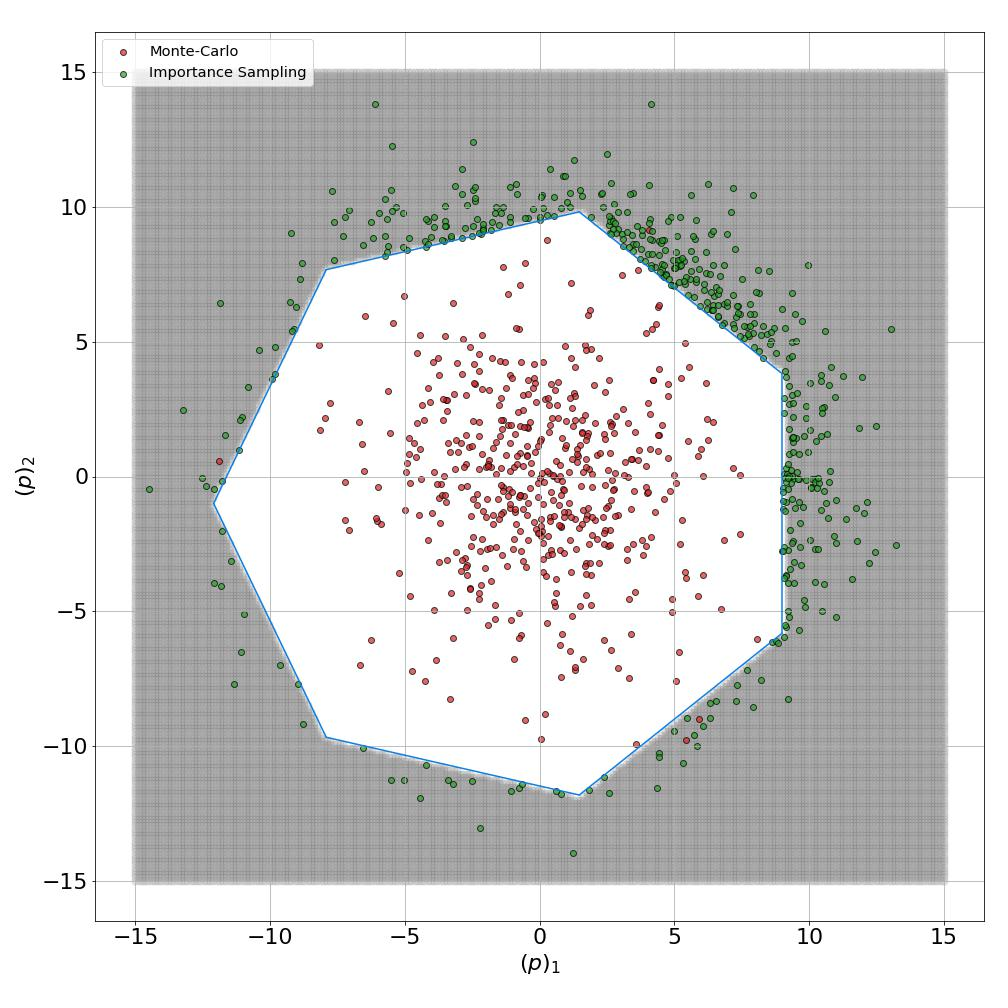
\includegraphics[width=.8\textwidth]{Dissertation/images/dc_stochastic_approx/conditioned_vs_MC (1).jpg}
  \caption{Sample difference between those produced by importance sampling and those by Monte-Carlo sampling.}
  \label{fig:conv_vs_MC-dc}
  
\end{figure}

\subsection{Scenario Approximation with Importance Sampling}

In this section, we present a scenario approximation for the chance-constrained optimal power flow with a set of scenarios generated by the ALOE algorithm~\cite{owen2019importance}. A particular advantage of this approach is that every scenario is generated outside of $\mathcal{P}_{\texttt{in}}$. The latter substantially improves the accuracy and efficiency of the scenario approximation. In particular, we solve the following optimization problem instead of Problem~\eqref{eq:sc-opf-dc}: 
\begin{subequations} 
\label{eq:FinA-dc}
  \begin{equation}
  \min_x \; \textit{cost}(x)\nonumber
  \end{equation}
  \begin{equation}
  \hspace{-20mm}\textit{s. t. }\;\; p^{\min} \le x+\xi^t \le p^{\max}, \; 1\le t \le N\label{eq:FinA-a-dc}
  \end{equation}
  \begin{equation}
   \hspace{11mm} |\theta_i(\xi^t) - \theta_j(\xi^t)| \le {\bar \theta}_{ij}, (i, j)\in \mathcal{E}, \; 1\le t \le N\label{eq:FinA-b-dc}
  \end{equation}
  \begin{equation}
  \hspace{-19mm} x+\xi^t = B \theta(\xi^t), \; 1\le t \le N\label{eq:FinA-c-dc}
  \end{equation}
  \begin{equation}
  \hspace{-50mm} x\in \mathcal{P}_{out} \label{eq:FinA-d-dc}
  \end{equation}
  \begin{equation}
  \hspace{-32mm} \xi^1, \xi^2, \dots, \xi^N\sim D \label{eq:FinA-e-dc},
  \end{equation}
\end{subequations} 
where $D$ is the probability distribution defined by Eq.~\eqref{eq:q_d-dc}. 

Notice, that sampling from distribution $D$ allows to efficiently generate scenarios outside of the polytope $\mathcal{P}_{\texttt{in}}$. However, they follow distribution $D$ instead of $\xi\sim \mathcal{N}(0, \Sigma) \textit{s. t. } \xi\not\in \mathcal{P}_{\texttt{in}}$. As these distributions are close to each other, Theorem~\ref{thm:80-dc} establishes efficient complexity bounds for the scenario approximation with importance sampling. 

\begin{theorem}\label{thm:80-dc}
Let $\bar x_N$ be a unique solution of the Scenario optimization Problem~\eqref{eq:FinA-dc} with $N$ i.i.d. samples follow distribution $D$. Moreover, assume that for any $N$ the assumption \ref{asmp:10-dc} is fulfilled. Then for any $\delta \in (0,1)$ and any~$\eta \in (0, 1/2]$, $\bar x_N$ is also a solution for the chance-constrained optimal power flow Problem~\eqref{eq:JCC-OPF-dc} with probability at least $1-\delta$ if 
\begin{align*}
  N \ge \left\lceil 2M\frac{(1-\pi)\ln \frac{1}{\delta}}{\eta} + 2d + 2d M(1-\pi) \frac{\ln\frac{2M(1-\pi)}{\eta}}{\eta} \right\rceil, 
\end{align*} 
where $d$ is a dimension of the problem and $\pi$ is a probability of a random scenario $\xi$ to belong to $\mathcal{P}_{\texttt{in}}$, $\pi < 1$, and constant $M$ is defined by Theorem~\ref{thm:50-dc}.
\end{theorem}
\begin{proof}
The proof is similar to the one of Theorem~\ref{thm:40-dc}. Application of theorem \ref{thm:50-dc} allows to upper-bound the probability of an event in measure $D$ with respect to its probability in measure $\mathcal{N}(0,\Sigma) \textit{s. t. } \xi\not\in\mathcal{P}_{\texttt{in}}$. 
\end{proof}

We emphasize that Theorem \ref{thm:40-dc} is a key theoretical result demonstrating a potential reduction in the number of samples. The latter is possible if scenarios are from a distribution such that a specific subset of its domain $\mathcal{P}_{\texttt{in}}$ has measure zero. Although, it is not possible to sample directly from such distribution. On the other hand, one can propose a mixture distribution to tackle this problem. In this case, Theorem \ref{thm:50-dc} is a practical statement that allows one to analyze the scenario approximation complexity constructed with scenarios from a mixture distribution.


\section{Empirical Study}\label{sec:emp-dc}
We compare our importance sampling-based approach (referred to as SA-IS) with the classical scenario approximation (SA)~\cite{calafiore2006scenario} over real and simulated test cases.
Empirical results justify our theoretical results: \emph{importance sampling based CC-OPF required much fewer samples to achieve a highly reliable solution than classical scenario approximation.} 

We limit the empirical setting to considering Gaussian distributions and linear feasibility constraints only.
%We omit detailed comparison with other importance sampling strategies \cite{genz2020package,lukashevich2021power,bugallo2017adaptive} when generating scenarios because of the chapter space limitation and for the sake of empirical study clarity. 
A profound discussion on the efficiency of importance samplers is given in~\cite{lukashevich2021power}.
\subsection{Implementation details} We use Python 3.9. and pandapower 2.8.0~\cite{thurner2018pandapower} on MacBook Pro (M1 Max, 64 GB RAM). In the experiments, the computational time for each case does not exceed five minutes, which makes it applicable for the operational practice. Our code is available online on Github~\footnote{https://github.com/vjugor1/IS-SA}. When solving the optimization problem, we use CVX~\cite{diamond2016cvxpy} and GLPK~\cite{GLPK} optimization solvers. 
\begin{figure}[!t]
  \centering
  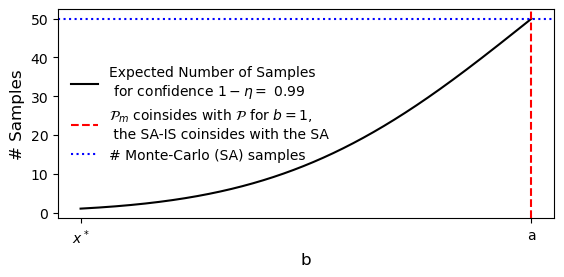
\includegraphics[width=.85\textwidth]{Dissertation/images/dc_stochastic_approx/figure120.png}
  \caption{
  Feasibility of the scenario approximation with importance sampling depending on the size of $\mathcal{P}_{out}= \{x: x\le b\}$, where $a \geq b\geq x^* =a - \Phi^{-1}(1-\eta)$. The more accurate approximation $\mathcal{P}_{out}$ is, the smaller is the number of samples required by the SA-IS algorithm.}
  \label{fig:80-dc}
  
\end{figure}

\subsection{Test Cases and Numerical Results}
\paragraph{Synthetic Example}
For elucidation of the theory, we first study the efficiency of importance sampling based scenarios over a one dimensional test case:
\begin{align*}
  \max\; & x\\
  \textit{s. t. } & \mathbb{P}_\xi(x+\xi \le a) \ge 1-\eta, \xi\sim \mathcal{N}(0,1)
\end{align*}
for $0 < \eta < 1/2$ and a positive constant $a$. In this case, the chance-constrained optimization problem admits an exact solution, $x^* = a - \Phi^{-1}(1-\eta)$. 

The polytopes $\mathcal{P}_{out}$ and $\mathcal{P}_{\texttt{in}}$ are $\{x: x\le x^*\}$ and $\{\xi: \xi \leq \Phi^{-1}(1-\eta)\}$ respectively. To illustrate the role of an approximation $\mathcal{P}_{out}$, $x^* \in \mathcal{P}_{out} \in \mathcal{P}$, we consider different polytopes $\mathcal{P}^b_{m} = \{x: x\le b\}$ and corresponding polytope $\mathcal{P}_{\texttt{in}}^b = \{\xi: \xi \leq a - b\}$, $a - b \le \Phi^{-1}(1-\eta)$.  

Figure~\ref{fig:80-dc} illustrates that the efficiency of sampling improves (i.e., less number of samples needed) as the polytope $\mathcal{P}_{out}$ better approximates $\mathcal{P}_{\texttt{in}}(0)$. Indeed, the probability of a sample from the nominal distribution outside of $\mathcal{P}_{\texttt{in}}^b$ being also outside $\mathcal{P}_{\texttt{in}}$ is proportional to $\Phi(a-b)$, which becomes negligible as $a-b$ decays and leads to a high number of samples. Note, that we reach the standard scenario approximation when $b = a$ and get the best possible approximation for $a-b = \Phi^{-1}(1-\eta)$. 


% \deep{Is the figure plotting a theoretical result..then state the analytical formula that is being depicted}
% \yury{I misunderstand what do you mean guys..}
% \sasha{the formula for this curve is needed, since it is obvously comes from Campi's theory (the plot)}

Our approach crucially relies on a non-conservative/tight approximation of the joint chance-constrained feasible set is crucial for the success of the importance sampling approach, as discussed next for power grid test cases. 

\begin{landscape}
\begin{table*}[t]
\caption{Number of SA-IS and SA samples required to reach reliability level $1-\hat{\delta} = 0.99$ in CC-OPF with confidence threshold $1-\eta$. }
    \centering
        \begin{tabular}{|lrrll|rll|l|}
        \toprule
           Case &  $\eta$ &  SA No &  SA Cost &   SA $(\mathbb{P}_N)$ &  IS-SA No & IS-SA Cost & IS-SA $(\mathbb{P}_N)$ & DC-OPF Cost \\
        \midrule
         grid30 &    0.05 &    160 & 5.89e+03 & 9.82e-01$\pm$7.09e-03 &        \textbf{60} &   5.87e+03 &  9.80e-01$\pm$8.86e-03 &    5.67e+03 \\
         grid57 &    0.05 &    210 & 2.52e+04 & 9.78e-01$\pm$8.95e-03 &       \textbf{160} &   2.52e+04 &  9.89e-01$\pm$7.71e-03 &    2.50e+04 \\
        grid118 &    0.05 &   1300 & 8.72e+04 & 9.68e-01$\pm$4.18e-03 &      \textbf{1050} &   8.72e+04 &  9.68e-01$\pm$4.16e-03 &    8.48e+04 \\
        grid300 &    0.05 &   1550 & 4.72e+05 & 9.63e-01$\pm$4.36e-03 &      \textbf{1250} &   4.72e+05 &  9.62e-01$\pm$3.97e-03 &    4.71e+05 \\
        \midrule
         grid30 &    0.01 &    800 & 5.94e+03 & 9.96e-01$\pm$1.83e-03 &       \textbf{300} &   5.96e+03 &  9.99e-01$\pm$6.57e-04 &    5.67e+03 \\
         grid57 &    0.01 &   1300 & 2.52e+04 & 9.96e-01$\pm$1.55e-03 &       \textbf{300} &   2.53e+04 &  9.97e-01$\pm$1.88e-03 &    2.50e+04 \\
        grid118 &    0.01 &   6000 & 8.74e+04 & 9.93e-01$\pm$1.16e-03 &      \textbf{3600} &   8.74e+04 &  9.94e-01$\pm$9.11e-04 &    8.48e+04 \\
        grid300 &    0.01 &   9000 & 4.72e+05 & 9.93e-01$\pm$8.42e-04 &      \textbf{4500} &   4.72e+05 &  9.92e-01$\pm$9.53e-04 &    4.71e+05 \\
        \bottomrule
        \end{tabular}
    \label{tab:summary_results-dc}
\end{table*}
\end{landscape}

\paragraph{Power grid test cases}
We address the scenario-based chance-constrained optimal power flow problem (CC-OPF) under Gaussian fluctuations in four different test cases (IEEE 30, IEEE 57, IEEE 118 and IEEE 300 bus systems with 30, 57, 118 and 300 buses/nodes, respectively). For all considered cases, we assume the power generation and consumption level fluctuate with the standard deviation of 0.07 of its nominal value. 

To demonstrate the practical benefits of importance sampling (SA-IS) versus standard scenario approximation (SA), we compare their respective number of samples $N$ needed to solve CC-OPF for different test cases, given prescribed $\eta,~\delta$. As stated in theorems in Section \ref{sec:algo-dc}, $1-\eta$ is the required \emph{confidence threshold} for constraint feasibility (of Joint Chance Constraint) by a solution, while $1-\delta$ is the required reliability of the Scenario Approximation's solution obtained.


We consider the setting of fixed confidence threshold $1-\eta$ and $N$, the number of samples used in CC-OPF (with SA-IS or SA), and determine their effect on empirical reliability $1-\hat{\delta}$ using Algorithm \ref{alg:estimate_delta-dc}. In Algorithm \ref{alg:estimate_delta-dc}, we independently form $L=100$ different scenario approximation problems, each with $N$ scenarios constructed using SA or SA-IS. We thus obtain $L$ different solutions $(x^*_N)_l, ~ l=1, \dots, L$. Using separately generated $10^4$ Monte Carlo samples of uncertainty for each $(x^*_N)_l$, we estimate each solution's probability of constraint satisfaction $(\hat{\mathbb{P}}_N)_l$. The estimated reliability $1-\hat{\delta}$ is then given by the fraction of $L$ $(x^*_N)_l$ solutions with $(\hat{\mathbb{P}}_N)_l \geq 1 - \eta$. 

\begin{algorithm}[ht]
\SetKwInOut{Input}{input}
\SetKwRepeat{Do}{do}{while}
% \SetKwInOut{Output}{output}
\caption{Reliability $1-\hat{\delta}$ -- an empirical estimate}\label{alg:estimate_delta-dc}
\Input{$L$ -- number of trials, DC-OPF problem parameters, $\eta$ -- confidence level, $N_0$ -- initial size of scenario approximation, $N_{\max}$ -- maximal size of scenario approximation}
$N \gets N_0$\;
$\hat{ \boldsymbol \delta}$ -- storage for $\hat{\delta}_N$\;
\Do{$N \leq N_{\max}$}
{
     $C_N \gets 0$ -- feasibility counter\;
     $l \gets 1$\;
    \Do{$l \leq L$}{
        Obtain $(x^*_N)_l$ -- scenario approximation with $N$ samples (using SA-IS or SA) \;
        Estimate constraint satisfaction probability $(\hat{\mathbb{P}}_N)_l$ using Monte Carlo samples.\label{alg:estimate_delta:phat_N_l-dc}\;
        \uIf{$(\hat{\mathbb{P}}_N)_l \geq 1 - \eta$}{
            $C_N \gets C_N +1$
        }
        }
    $1-\hat{\delta}_N \gets C_N / L$ -- fraction of trials turned out to be feasible \;
    Append $\hat{\delta}_N$ to $\hat{ \boldsymbol \delta}$ \;
    $n  \gets n + N_{\max}/ 10$\;
}
\Return $\hat{ \boldsymbol \delta}$
\end{algorithm}

% \begin{algorithm}[ht]
% \caption{Reliability $1-\hat{\delta}$ -- an empirical estimate}\label{alg:estimate_delta}
% \begin{algorithmic}
% \Require $L$ -- number of trials, DC-OPF problem parameters, $\eta$ -- confidence level, $N_0$ -- initial size of scenario approximation, $N_{\max}$ -- maximal size of scenario approximation
% \State $N \gets N_0$
% \State $\hat{ \boldsymbol \delta}$ -- storage for $\hat{\delta}_N$
% \While{$N \leq N_{\max}$}
%     \State $C_N \gets 0$ -- feasibility counter
%     \State $l \gets 1$
%     \While{$l \leq L$}
%         \State Obtain $(x^*_N)_l$ -- scenario approximation with $N$ samples (using SA-IS or SA)
%         \State Estimate constraint satisfaction probability $(\hat{\mathbb{P}}_N)_l$ using Monte Carlo samples. \label{alg:estimate_delta:phat_N_l}
%         \If{$(\hat{\mathbb{P}}_N)_l \geq 1 - \eta$}
%             $C_N \gets C_N +1$
%         \EndIf
%     \EndWhile
%     \State $1-\hat{\delta}_N \gets C_N / L$ -- fraction of trials turned out to be feasible
%     \State Append $\hat{\delta}_N$ to $\hat{ \boldsymbol \delta}$
%     \State $n  \gets n + N_{\max}/ 10$
% \EndWhile
% \State \Return $\hat{ \boldsymbol \delta}$
% \end{algorithmic}

% \end{algorithm}

Table~\ref{tab:summary_results-dc} summarizes the number of samples needed using SA and SA-IS to ensure an empirical reliability of $0.99$, for two confidence thresholds $1-\eta$ ($0.95$ and $0.99$). The number of scenarios required for target reliability were obtained empirically, iterating over a predefined grid for $N$ with the step of $10$. The confidence threshold $1-\eta$ is estimated using Monte Carlo samples (out of sample) and empirical reliability is computed by averaging over $L=100$ independent CC-OPF problem instances as stated in Algorithm~\ref{alg:estimate_delta-dc}. The costs of solutions obtained are depicted alongside with the corresponding costs of deterministic DC-OPF solution. It is clear that SA-IS requires much less samples compared to SA, while maintaning the same reliability of the solution. Our experiments show that SA-IS requires much fewer samples to provide a reliable CC-OPF feasible solution while maintaining the same cost for each test case compared to CC-OPF with SA. The improvement in the number of scenarios is bigger for the higher confidence threshold value ($1-\eta=0.99$).

The reliability analysis of approximations' solutions is presented in Figures \ref{fig:spreads-dc}, \ref{fig:empiricals-dc}, the latter illustrates empirical reliability ($1-\hat{\delta}$) and the former illustrates the spread of constraint feasibility $(\hat{\mathbb{P}}_N)_l$ for CC-OPF ($1-\eta =.99$) for IEEE 300 bus and IEEE 118 bus systems. The three cases correspond to samples in CC-OPF being drawn by SA, SA-IS and SA-O. The empirical estimates are computed with $L = 100$ optimization instances (for $1-\hat{\delta}$), and $N_{MC}=10^4$ Monte-Carlo samples for each instance to determine constraint validation (for box-plot of $(\hat{\mathbb{P}}_N)_l$), as described in Algorithm~\ref{alg:estimate_delta-dc}. 
Colored boxes stands for the 25\% -- 75\% interquantile range (IQR). Diamonds shows samples outside of the $\pm 1.5*\text{IQR}$. 
Note that both in reliability, and the IRQ of constraint feasibility, SA-IS requires much less number of samples compared to SA or~SA-O.

We illustrate the dependence between empirical reliability $1-\hat{\delta}$ and $N$ over a range of values for the IEEE 118 bus system in Fig. \ref{fig:ieee118reliability-dc}. Here, we keep a confidence threshold of joint chance constraint feasibility $1-\eta =0.99$. In addition to SA-IS and SA, we also consider an intermediate setting - Scenario Approximation with Polygon-Set (SA-O), as described in Eq.~\eqref{eq:Fin-dc}. 

Compared to SA, SA-O includes the inner approximation constraints $x \in \mathcal{P}_{out}$. However, unlike SA-IS, SA-O does not involve importance sampling-based samples. It is clear from Fig.~\ref{fig:ieee118reliability-dc} that at all values of $N$, SA-IS's reliability $1-\hat{\delta}$ is much higher than that of SA or SA-O. In fact, for $3500\leq N \leq 4000$, the SA-IS is around ten times more reliable than SA. As a result, the solution of SA-IS also becomes conservative faster (highlighted by the decrease in slope at higher reliability). On the other hand, SA and SA-O have almost similar reliability, which follows from Theorem \ref{thm:20-dc}. 

Finally, for the same $L$ optimization instances used for Fig.~\ref{fig:ieee118reliability-dc}, we present box-plots for the spread of $(\hat{\mathbb{P}}_N)_l$ for different $N$, in Fig.~\ref{fig:ieee118conservatism-dc}. Here, $(\hat{\mathbb{P}}_N)_l$ is the probability of constraint satisfaction, empirically estimated using $10^4$ Monte Carlo separately generated samples as stated in Algorithm \ref{alg:estimate_delta-dc}. Note that SA-IS reaches a higher reliability level ($1-\hat{\delta}$) at a fewer number of samples $N$, observed when almost all of the box is above the $1-\eta$ threshold. The boxplots also indicate that the variance in the obtained solution's chance-constraint feasibility reduces faster for SA-IS, noted by thinner boxplots and lack of outliers, compared to SA and SA-O.

\begin{figure*}[hbt]
\centering
\begin{subfigure}{.8\textwidth}
  \centering
  % include first image
  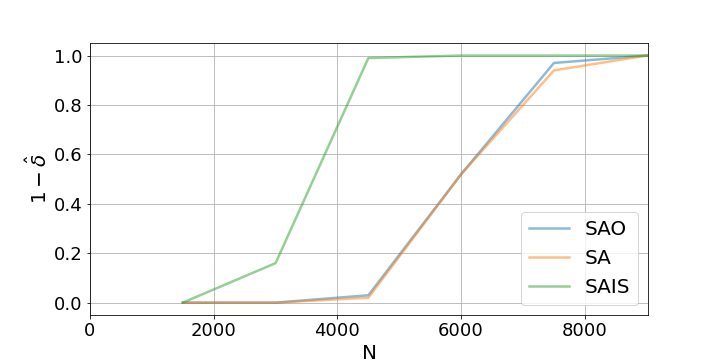
\includegraphics[width=0.99\linewidth]{Dissertation/images/dc_stochastic_approx/case300/1_beta_N_12000_eta_001.png}~~~~~~\hfill
  \caption{IEEE 300 bus system.}
  \label{fig:ieee300reliability-dc}
\end{subfigure}

\begin{subfigure}{.8\textwidth}
  \centering
  % include first image
  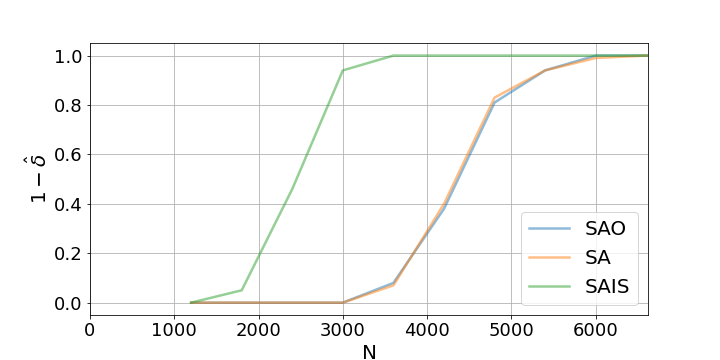
\includegraphics[width=0.99\linewidth]{Dissertation/images/dc_stochastic_approx/ieee118/1_beta_N_7800_eta_001.png}~~~~~~\hfill
  \caption{IEEE 118 bus system.}
  \label{fig:ieee118reliability-dc}
\end{subfigure}
\caption{Empirical reliability ($1-\hat{\delta}$) versus number of samples in \\CC-OPF ($N$).}
\label{fig:empiricals-dc}
\end{figure*}

\begin{figure*}[hbt]
\centering
\begin{subfigure}{.8\textwidth}
  \centering
  % include second image
  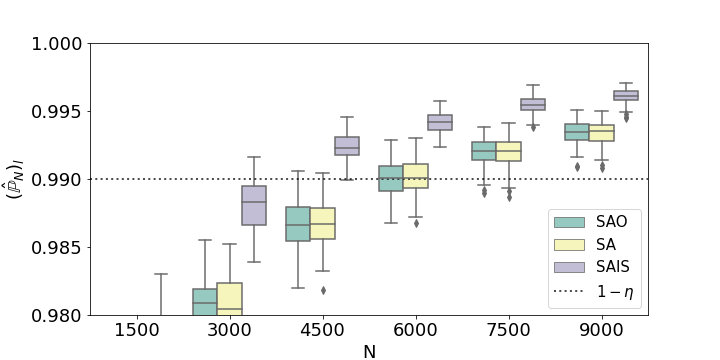
\includegraphics[width=0.99\linewidth]{Dissertation/images/dc_stochastic_approx/case300/boxplot_J_N_9000_eta_001.png}
  \caption{IEEE 300 bus system.}
  \label{fig:ieee300conservatism-dc}
\end{subfigure}

\begin{subfigure}{.8\textwidth}
  \centering
  % include second image
  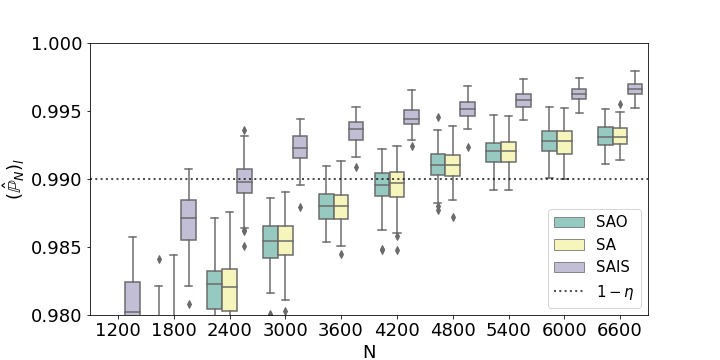
\includegraphics[width=0.99\linewidth]{Dissertation/images/dc_stochastic_approx/ieee118/boxplot_J_N_6600_eta_001.png}
  \caption{IEEE 118 bus system.}
  \label{fig:ieee118conservatism-dc}
\end{subfigure}
\caption{Spread of probability of constraint feasibility ($(\hat{\mathbb{P}}_N)_l$) versus number of samples in CC-OPF ($N$).}
\label{fig:spreads-dc}
\end{figure*}

Finally, we address the question if the total computational time for SA-IS is better than for classical SA. First, we address the amount of time required to generate samples for classical Monte-Carlo SA, and those for IS-SA using Importance Sampling technique. Next, we analyze how to much time totally is required to obtain $1-\hat{\delta}=0.99$-reliable solution. For such experiment we consider generating samples for IEEE-30 power system. 

In order to compare preprocessing step, i.e., sampling generation step, we generate $N=50, 150, 250, 350, 450$ samples with ALOE, and the same amount of samples from multivariate normal distribution. For each $N$ we repeat generation 15 times to obtain statistics on execution time. Similarly, with the same strategy we generate the samples for each $N$ and solve the scenario approximation and collect execution time, repeating for 15 times. 
The execution time of the preprocessing step comparison is visualized in Figure \ref{fig:profile_generate_samples-dc}. On the right Figure, vertical dashed lines indicate number of samples that are sufficient to reach $1-\hat{\delta}=0.99$ reliability level for $\eta=0.05$, see Table \ref{tab:summary_results-dc}. Horizontal dot-dashed lines demonstrate the amount of time spent on average over 15 runs. From this figure, one can observe that ALOE is a more time consuming procedure. However, one can observe that the time required to solve scenario approximations together with preprocessing does not differ significantly for IS-SA and SA -- see Figure \ref{fig:profile_scenario_approx-dc}. The latter figure also shows that the computational time required to obtain the same reliability level is five times less for SA-IS (the number of samples are taken from Table \ref{tab:summary_results-dc}, case IEEE-30, $\eta=0.05$.)

\begin{figure*}[hbt]
\centering
\begin{subfigure}{.8\textwidth}
  \centering
  % include first image
  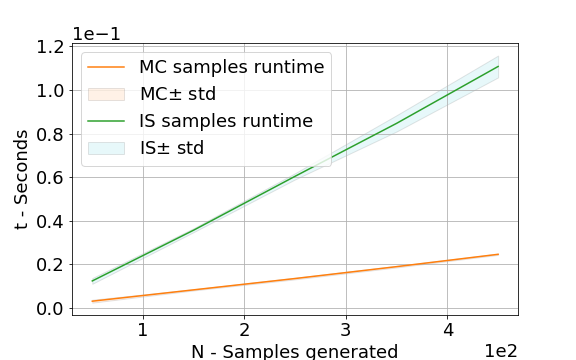
\includegraphics[width=0.9\linewidth]{Dissertation/images/dc_stochastic_approx/profiling_samplig.png}~~~~~~\hfill
  \caption{Sample generation.}
  \label{fig:profile_generate_samples-dc}
\end{subfigure}
\begin{subfigure}{.8\textwidth}
  \centering
  % include second image
  \hspace{-10mm}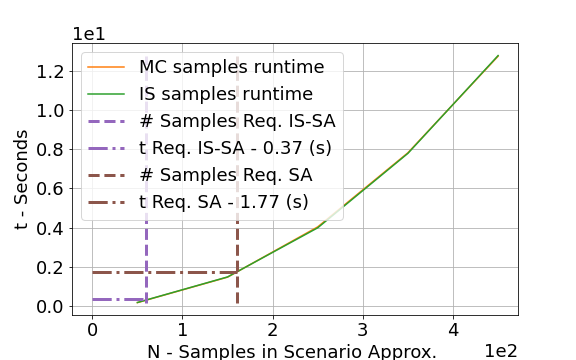
\includegraphics[width=0.9\linewidth]{Dissertation/images/dc_stochastic_approx/profiling_approx_sol.png}
  \caption{Samples preparation, assembling scenario approximation and solving the latter, formed for different $N$.}
  \label{fig:profile_scenario_approx-dc}
\end{subfigure}
\caption{Computational time required to complete prepocessing step \ref{fig:profile_generate_samples-dc} and solve corresponding scenario approximations \ref{fig:profile_scenario_approx-dc} for IEEE-30 case. }
\label{fig:profiling-dc}
\end{figure*}


\section{Conclusion}
\label{sec:conclusion-dc}
In this chapter, we investigated the scenario approximation for the chance-constrained optimal power flow. We showed that the importance sampling technique used for scenario generation leads to a better accuracy. Moreover, the numerical complexity is much lower in theory and practice for stochastic OPF. 

The theoretical study indicates the benefit of using violative samples. The results are presented and proven alongside numerical experiments that indicate a significant reduction of sample size in scenario approximation required to reach a high reliability level. Finally, the approach can be extended to automated real-time control of bulk power systems. 